\section{Provenance Analysis}
\label{sec:provenance-analysis}

The graph at \texttt{doc/provenance.ttl} is a queryable structure
whose health \emph{is} the audit pass on \textbf{Reusable}
(\S\ref{sec:axes}). Figure~\ref{fig:provenance-topology} renders
the schema with live instance counts read at compile time. Four
diagnostic SPARQL queries (rung distribution, section-to-claim
coverage, source invocation strength, activity timeline) and the
auto-generated tables they produce are walked in
\companionref{sec:appendix-provenance-analysis}{Appendix~E:
Provenance Analysis --- Queries and Worked Numbers}.

\begin{figure}[!h]
\centering
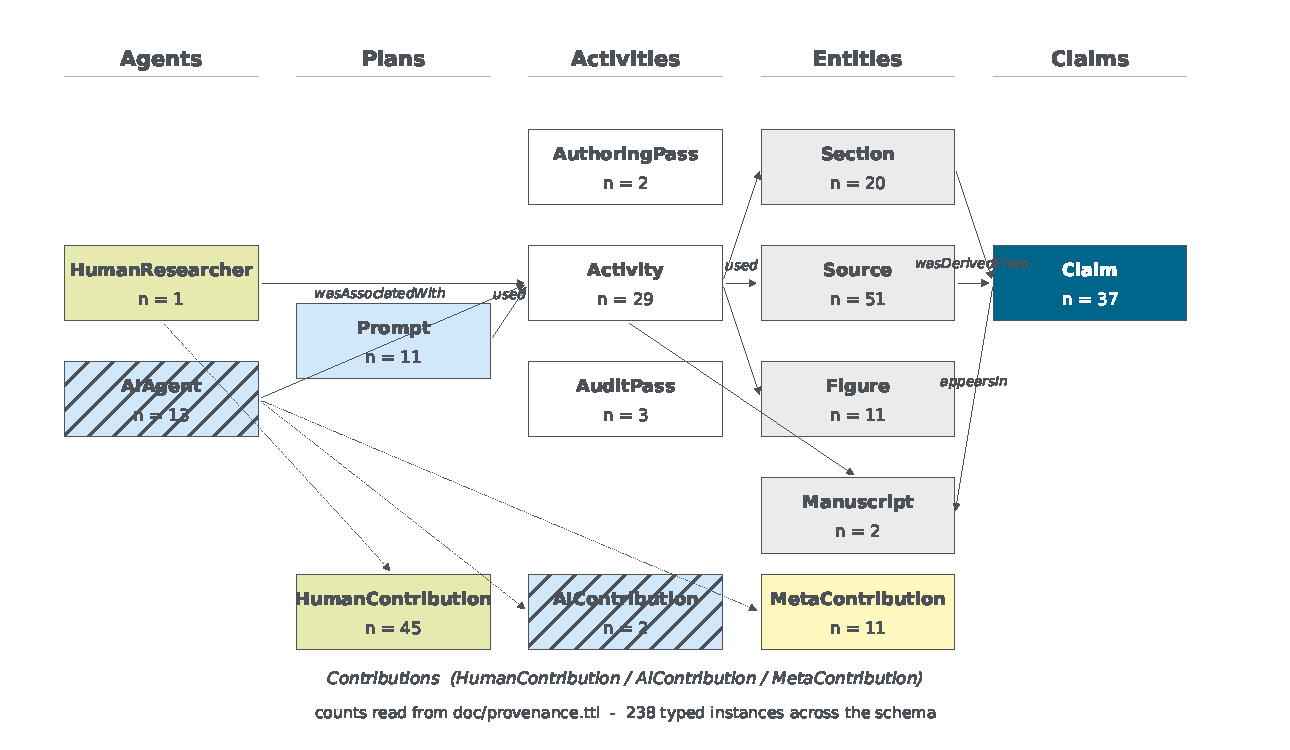
\includegraphics[width=0.96\linewidth]{figures/provenance-topology.pdf}
\caption{Shape of the F(AI)\textsuperscript{2}R provenance graph,
read from the live \texttt{doc/provenance.ttl} at compile time.
Five PROV-O lanes (Agents, Plans, Activities, Entities, Claims)
plus a Contribution satellite band; each node is decorated with
its current instance count.}
\label{fig:provenance-topology}
\end{figure}

The queries are diagnostic, not exhaustive. They surface the
failure modes of \S\ref{sec:failure-modes} with a graph signature
(ghost citations, prose--graph drift, sections without curated
claims) and explicitly do not surface \textbf{semantic} drift ---
a claim correctly recorded but whose prose has shifted away from
its evidence --- which is the readability scrutinizer's job
(\S\ref{sec:pipeline}). A live interactive view is published at
\href{https://noheton.github.io/f-ai-r/provenance.html}{the
\textbf{Provenance} tab of the public site}; the populated
verification-ladder FSM is on the conference poster
(\texttt{slides/poster-A0.tex}).
